\documentclass[a4paper, 12pt]{report}

% PACKAGES %%%%%%%%%%%%%%%%%%%%%%%%%%%%%%%%%%%%%%%%%%%%%%%%%%%%%%%%%%%%%%%%%%%
\usepackage{lipsum} 
\usepackage[utf8]{inputenc}
\usepackage{graphicx}
\usepackage[justification=centering]{caption} % All captions will be centered. 
\usepackage{url} % To include in URL in reference. 
\usepackage[nottoc]{tocbibind} %Includes "References" in the table of contents
\usepackage{setspace} % To add linespace
\usepackage{tocloft} % To change formatting of main list. 
\usepackage{titlesec} % Customize chapter title: Make it centered. 
\usepackage[a4paper, left=1.5in, right=1in, top=1in, bottom=1in]{geometry}
\usepackage{float} % To use ht with table. To fix table position. 
\usepackage{minted} % For code. 
\usepackage[skip=12pt]{parskip} % Indentation between paragraphs
\usepackage[style=long,nonumberlist,toc,xindy,acronym,nomain]{glossaries}


%  TWEAKS %%%%%%%%%%%%%%%%%%%%%%%%%%%%%%%%%%%%%%%%%%%%%%%%%%%%%%%%%%%%%%%%%%%%
% Center the chapter title and make it uppercase. 
\titleformat{\chapter}[display]
  {\normalfont\Large\bfseries\centering}
  {CHAPTER \thechapter}{20pt}{\Large\uppercase}
% To fix table position using ht. package: float
\restylefloat{table}
\makeglossaries


% VARIABLES %%%%%%%%%%%%%%%%%%%%%%%%%%%%%%%%%%%%%%%%%%%%%%%%%%%%%%%%%%%%%%%%%%
\newcommand\cTitle{PROJECT TITLE}

\newcommand\cMembOne{MEMBER ONE}
\newcommand\cMembTwo{MEMBER TWO}
\newcommand\cMembThree{MEMBER THREE}
\newcommand\cMembFour{MEMBER FOUR}

\newcommand\cMembOneRegNo{PKD19XXXXX}
\newcommand\cMembTwoRegNo{PKD19XXXXX}
\newcommand\cMembThreeRegNo{PKD19XXXXX}
\newcommand\cMembFourRegNo{PKD19\-XXXXX}

\newcommand\cGuide{GUIDE}
\newcommand\cHod{HOD}
\newcommand\cPrincipal{PRINCIPAL}
\newcommand\cCordOne{COORDINATOR-ONE}
\newcommand\cCordTwo{COORDINATOR-TWO}

\newcommand\cMonthAndYear{December 2022}


\begin{document}
\onehalfspacing

% COVER PAGES %%%%%%%%%%%%%%%%%%%%%%%%%%%%%%%%%%%%%%%%%%%%%%%%%%%%%%%%%%%%%%%
\begin{titlepage}
  \newgeometry{left=1in, right=1in, top=1in, bottom=1in}
  \begin{center}
    \textbf{\Large\cTitle}\\
    \vfill
    A PROJECT REPORT\\
    \vfill
    submitted by\\
    \vfill
    
    \textbf{\MakeUppercase{\cMembOne (\cMembOneRegNo)} } \\
    \textbf{\MakeUppercase{\cMembTwo (\cMembTwoRegNo)} } \\
    \textbf{\MakeUppercase{\cMembThree (\cMembThreeRegNo)} } \\
    \textbf{\MakeUppercase{\cMembFour (\cMembFourRegNo)}  } \\
    
    \vfill
    to\\
    the APJ Abdul Kalam Technological University\\
    \vfill
    in partial fulfilment of the requirements for the award of the Degree\\
    of\\
    \emph{
        Bachelor of Technology\\
        in\\
        Information Technology
    }
    \vfill
    
\includegraphics[scale=.3]{"covers/images/logo_gecp.png"}
    \vfill
    \textbf{Department of Information Technology\\
      Government Engineering College Palakkad\\
      Sreekrishnapuram, Palakkad-678633}\\
    \cMonthAndYear
  \end{center}
  \restoregeometry
\end{titlepage}
\begin{titlepage}
  \begin{center}
    \textbf{\Large\cTitle}\\
    \vfill
    AN INTERIM PROJECT REPORT\\
    \vfill
    submitted by\\
    \vfill
    
    \textbf{\MakeUppercase{\cMembOne (\cMembOneRegNo)} } \\
    \textbf{\MakeUppercase{\cMembTwo (\cMembTwoRegNo)} } \\
    \textbf{\MakeUppercase{\cMembThree (\cMembThreeRegNo)} } \\
    \textbf{\MakeUppercase{\cMembFour (\cMembFourRegNo)}  } \\
    
    \vfill
    to\\
    the APJ Abdul Kalam Technological University\\
    \vfill
    in partial fulfilment of the requirements for the award of the Degree\\
    of\\
    \emph{
        Bachelor of Technology\\
        in\\
        Information Technology
    }
    \vfill
    
\includegraphics[scale=.3]{"covers/images/logo_gecp.png"}
    \vfill
    \textbf{Department of Information Technology\\
      Government Engineering College Palakkad\\
      Sreekrishnapuram, Palakkad-678633}\\
    \cMonthAndYear
  \end{center}
\end{titlepage}
\begin{titlepage}
\chapter*{DECLARATION}
\thispagestyle{empty}

\noindent We hereby declare that the seminar report entitled "{\textbf{\cTitle}}" submitted by us to the APJ Abdul Kalam Technological University during the academic year 2022-23 in partial fulfilment of the requirements for the award of Degree of Bachelor of Technology in Information Technology is a record of bonafide seminar work carried out by us under the guidance and supervision of \cGuide. We further declare that the work reported in this project has not been submitted and will not be submitted, either in part or in full, for the award of any other degree or diploma in this institute or any other University.

\vspace{2cm}

\begin{flushright}
\textbf{\MakeUppercase{\cMembOne} (\cMembOneRegNo)} \\
\textbf{\MakeUppercase{\cMembTwo} (\cMembTwoRegNo)} \\ 
\textbf{\MakeUppercase{\cMembThree} (\cMembThreeRegNo)} \\
\textbf{\MakeUppercase{\cMembFour} (\cMembFourRegNo)}
\end{flushright}

\noindent Place: Sreekrishnapuram \\
Date: \today

\end{titlepage}
\begin{titlepage}
\vfill
\begin{center}
    \textbf{
    DEPARTMENT OF INFORMATION TECHNOLOGY\\ 
    GOVERNMENT ENGINEERING COLLEGE PALAKKAD\\ 
    SREEKRISHNAPURAM, PALAKKAD – 678633
    }
    
    \vspace{1cm}
    
    
\includegraphics[scale=0.3]{covers/images/logo_gecp.png}
    
    \vspace{1cm}
    
    \textbf{
        \Large{
            CERTIFICATE
        }
    }
    
\end{center}

\noindent This is to certify that the report entitled “\textbf{\cTitle}” submitted by \textbf{\MakeUppercase{\cMembOne} (\cMembOneRegNo)}, \textbf{\MakeUppercase{\cMembTwo} (\cMembTwoRegNo)}, \textbf{\MakeUppercase{\cMembThree} (\cMembThreeRegNo)}, and \textbf{\MakeUppercase{\cMembFour} (\cMembFourRegNo)},
to the APJ Abdul Kalam Technological University in partial fulfilment of the requirements for the award of the Degree of Bachelor of Technology in Information Technology is a bonafide record of the project work carried out by him under our guidance and supervision. This report in any form has not been submitted to any other Universities or institutes for any purpose.

\vspace{2cm}


\noindent GUIDE\hfill HEAD OF THE DEPARTMENT\\
\cGuide \hfill \cHod \\
Associate Professor \hfill Associate Professor\\
Dept. of Information Technology\ \hfill Dept. of Information Technology\\
% \begin{flushright}
%     \textbf{GUIDE \& HEAD OF THE DEPARTMENT}\\
%     \cHod \\
%     Associate Professor\\
%     Dept. of Information Technology\\
% \end{flushright}

\end{titlepage}



\renewcommand{\cftchappresnum}{Chapter }
\renewcommand\cftchapaftersnum{\hfill:\hfill}
\renewcommand\cftchapnumwidth{2.5cm}

  
\let\mtcontentsname\contentsname
\renewcommand\contentsname{\hfill \Large CONTENTS\hfill\null{}} % dummy text \null{} to center the TOC title. 

% Remove page number from TOC. Ref: https://tex.stackexchange.com/a/180877/193507
\pagestyle{empty}
{
  \renewcommand{\thispagestyle}[1]{}
  \tableofcontents
}
\clearpage
\pagestyle{plain}

\pagenumbering{roman}
\chapter*{\centering ACKNOWLEDGEMENT}
\addcontentsline{toc}{chapter}{ACKNOWLEDGEMENT} 

Many noble hearts contributed immense inspiration and support for the successful completion of the project. We are unable to express our gratitude in words to such individuals.

We would like to express our deep regard to \cPrincipal, Principal, Government Engineering College, Palakkad, for providing facilities throughout the works of our project. 

We take this opportunity to express our profound gratitude to \cHod, Head of the Department, Department of Information Technology, Government Engineering College, Palakkad, for providing permission and availing all required facilities for undertaking the project in a systematic way. We are extremely grateful to \cGuide, Associate Professor, Department of Information Technology, Government Engineering College, Palakkad, who guided us with his kind, ordinal and valuable suggestions. We pay our deep sense of gratitude to \cCordOne and \cCordTwo project coordinators, Department of Information Technology, Government Engineering College, Palakkad, for their valuable guidance, keen interest and encouragement at various stages of the project. We would also like to thank all the teaching and nonteaching staff of Department of Information Technology, Government Engineering College, Palakkad, for the sincere directions imparted and the cooperation in connection with the project. 

We will be failing in duty if we do not acknowledge with grateful thanks to the authors of the references and other literatures referred in this project. 

Last, but not the least, We take pleasant privilege in expressing our heartful thanks to our friends who were of precious help in completing this project.    
\chapter*{\centering ABSTRACT}
\addcontentsline{toc}{chapter}{ABSTRACT} 

\lipsum[1]
% tocloft package 
\renewcommand{\cftlottitlefont}{\hspace*{\fill}\Large\bfseries}
\renewcommand{\cftafterlottitle}{\hspace*{\fill}}

\renewcommand*\listtablename{LIST OF TABLES}
\listoftables
\thispagestyle{empty}
% \thispagestyle{empty} % uncomment to remove page number 
%  tocloft package 
\renewcommand{\cftloftitlefont}{\hspace*{\fill}\Large\bfseries}
\renewcommand{\cftafterloftitle}{\hspace*{\fill}}

\renewcommand*\listfigurename{\centering LIST OF FIGURES}
\listoffigures
% \thispagestyle{empty} % uncomment to remove page number
 
% ACRONYMS %%%%%%%%%%%%%%%%%%%%%%%%%%%%%%%%%%%%%%%%%%%%%%
\newacronym{sa}{SA}{Simple Abbr}



% PRINT GLOSSARY %%%%%%%%%%%%%%%%%%%%%%%%%%%%%%%%%%%%%%%%
\printglossary[type=\acronymtype, title=ABBREVIATIONS, toctitle=ABBREVIATIONS]


% CHAPTERS %%%%%%%%%%%%%%%%%%%%%%%%%%%%%%%%%%%%%%%%%%%%%%%%%%%%%%%%%%%%%%%%%
\pagenumbering{arabic} % Arabic numbers for contents
\chapter{Introduction}

\section{Figures}

Place your image in chapters/images folder. Refer \ref{fig:waterfall}
\begin{figure}
    \centering
    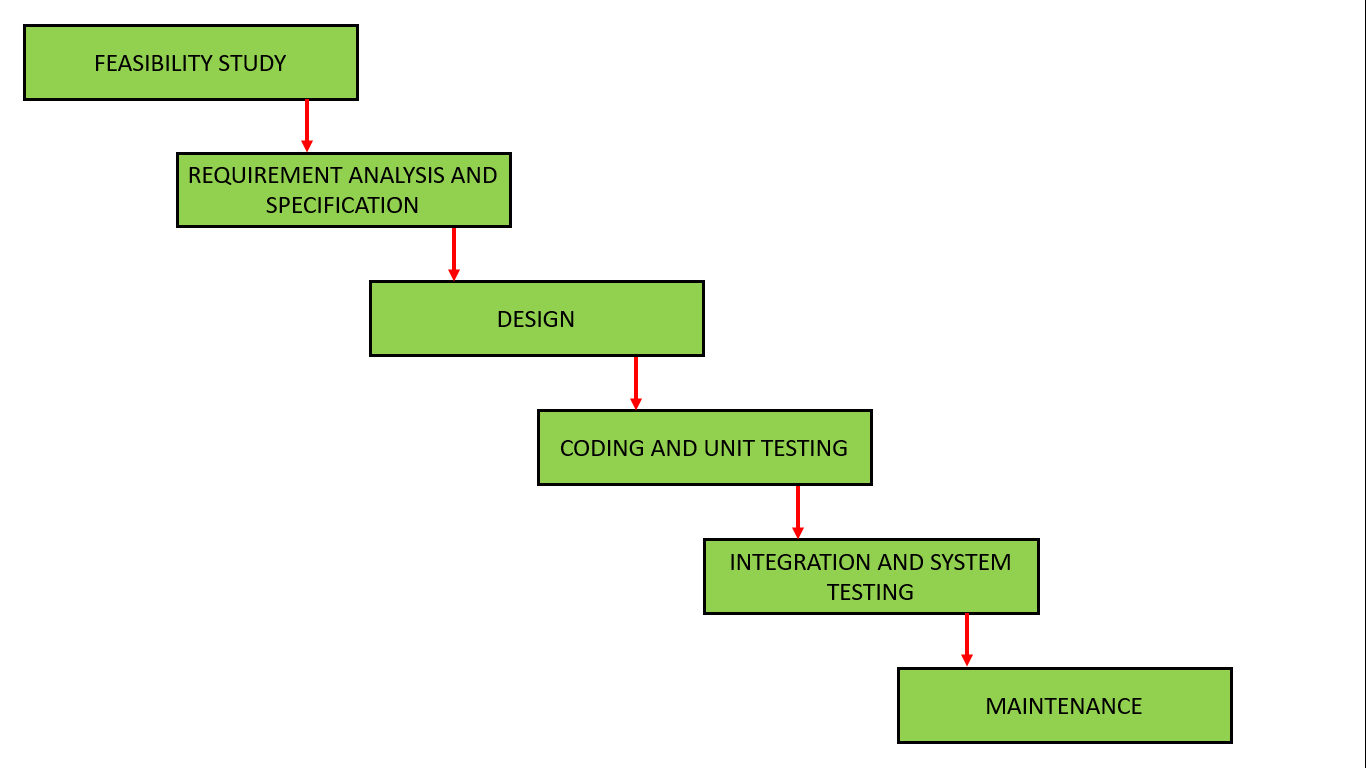
\includegraphics[scale=0.15]{chapters/images/waterfall.png}
    \caption{Various stages involved in the waterfall model}
    \label{fig:waterfall}
\end{figure}

\section{Code snippets}
Place your code snippets in codes folder. Refer \ref{fig:sample_code} 
\begin{figure}
    \begin{minted}{js}
function sample () {
    console.log("Sample code");
}
\end{minted}
    \caption{Sample function.}
    \label{fig:sample_code}
\end{figure}

\section{Tables}
\begin{table}[h!]
    \centering
    \begin{tabular}{l|l}
        A & B \\
        \hline 
        1 & 2 
    \end{tabular}
    \caption{Sample table}
    \label{tab:highlights}
\end{table}

\section{Abbreviations}
Create abbreviations in covers/abbreviations.tex file and refer them here using gls. Eg. Simple Abbr(\gls{sa})

\section{Footnotes}
You can add footnotes \footnote{Sample footnote}

\section{References}
Add BibTeX format bibliography entries in bib.bib and cite anywhere like this; \cite{sample_cite}


%  TWEAKS %%%%%%%%%%%%%%%%%%%%%%%%%%%%%%%%%%%%%%%%%%%%%%%%%%%%%%%%%%%%%%%%%%%%
% Center chapter title and make it uppercase. 
\titleformat{\chapter}[display]
  {\normalfont\Large\bfseries\centering}
  {CHAPTER \thechapter}{20pt}{\Large\uppercase}
% To fix table position using ht. package: float
\restylefloat{table}


% APPENDICES %%%%%%%%%%%%%%%%%%%%%%%%%%%%%%%%%%%%%%%%%%%%%%%%%%%%%%%%%%%%%%%
\appendix  

% BIBLIOGRAPHY %%%%%%%%%%%%%%%%%%%%%%%%%%%%%%%%%%%%%%%%%%%%%%%%%%%%%%%%%%%%%
\renewcommand{\bibname}{REFERENCES}
\bibliographystyle{plain}
\renewcommand{\thepage}{}
\bibliography{bib}


\end{document}
